\section{Experimental evaluation}\label{sec:experiment}
In this section, an experimental evaluation over X real-life event logs is reported.


\subsection{Re-sampling and test setup}
Time series are obtained by specifying a number of intervals (i.e. time steps in the DF series) using either equitemporal or equisize aggregation.
Time series algorithms are parametric and sensitive to sample size requirements \cite{hanke2001business}.
Depending on the number of parameters a model uses, a minimum size of at least 50 steps is not uncommon, although typically model performance should be monitored at a varying number of steps.
In the experimental evaluation, three different results will be given to study the impact of the number of steps. 
100 intervals are established and time series models are trained over the first quarter, the first two quarters, and first three quarters of data points to forecast the second, third, and fourth quarter of data points respectively.
This allows to both inspect the difference in result when only few data points are used, and whether there is a difference forecasting data points in the middle or towards the end of the trace.

Three widely-used event logs are used: the 2012 BPI challenge log\footnote{\url{https://doi.org/10.4121/uuid:3926db30-f712-4394-aebc-75976070e91f}}, the Sepsis cases event log\footnote{\url{https://doi.org/10.4121/uuid:915d2bfb-7e84-49ad-a286-dc35f063a460}}, and the Road Traffic Fine Management Process log\footnote{\url{https://doi.org/10.4121/uuid:270fd440-1057-4fb9-89a9-b699b47990f5}} (RTFMP) event log.
Each of these logs has a diverse set of characteristics in terms of case and activity volume, as well as average trace length as can be seen in Table \ref{tab:eventlogs}.
\begin{table}[htbp]
  \centering
    \begin{tabular}{lrrr}
    \toprule
    \textbf{Event log} & \multicolumn{1}{l}{\textbf{\# cases}} & \multicolumn{1}{l}{\textbf{\# activities}} & \multicolumn{1}{l}{\textbf{Average trace length}} \\
    \midrule
    \textbf{BPI 12} & 13,087 & 36    & 20.020 \\
    \textbf{Sepsis} & 1,050 & 16    & 14.490 \\
    \textbf{RTFMP} & 150,370 & 11    & 3.734 \\
    \bottomrule
    \end{tabular}%
  \caption{Overview of the characteristics of the event logs used in the experimental evaluation.}
  \label{tab:eventlogs}%
\end{table}%

An example of applying the equisize or equitemporal aggregation to the event logs with 100 intervals results in the DF time series of Figures \ref{fig:bpi12ts} to \ref{fig:rtfmpts} where the most frequently occurring activity pairs are included.
The equitemporal aggregation is based on a number of intervals over the whole time span of the event log.
When using this aggregation, a noticeable decline of DF pairs is visible towards the end of the series.
This phenomenon is typical in event logs, as processes typically have particular endpoint activity, e.g., the closure of a loan application event in the BPI 12 log.
The use of a cutoff of 50 for the most-frequently occurring DF pairs results in different time series as well.
For the BPI 12 log, the frequency of the 50th pair is still relatively high, while for the other event logs the frequency of the DF pair is low and close to 0, making the series unsuitable for analysis with white noise series analysis techniques that assume stationarity.
Ideally, every time series is tested using a stationarity test such as the Dickey-Fuller unit root test \cite{leybourne1995testing} and an appropriate lag order is established for differencing. 
Furthermore for each algorithm, especially ARIMA-based models, (partial) auto-correlation could establish the ideal $p$ and $q$ parameters.
However, for the sake of simplicity and to avoid tedious solutions where each activity pair has to have different parameters, various values are used for $p$, $d$, and $q$ and applied to all DF pairs where only the best-performing are reported below for comparison with the other time series techniques.

\begin{figure}[tb]
	\centering
	\subfigure[Most common DF - equisize]{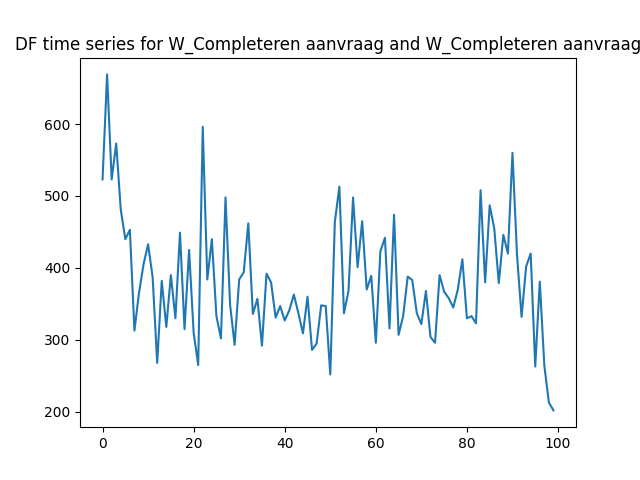
\includegraphics[width=0.49\textwidth]{./img/bpi12_1.png}}
	\subfigure[Most common DF - equitemp]{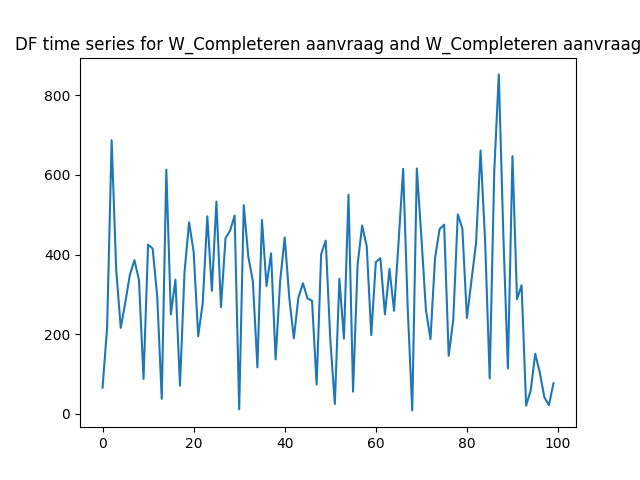
\includegraphics[width=0.49\textwidth]{./img/bpi12_1_t.png}}
	\caption{BPI 12}
	\label{fig:bpi12ts}
\end{figure}

\begin{figure}[tb]
	\centering
	\subfigure[Most common DF - equisize]{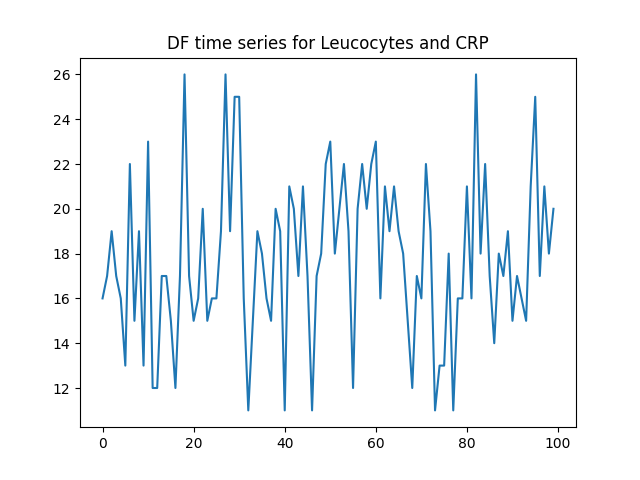
\includegraphics[width=0.49\textwidth]{./img/sepsis_1.png}}
	\subfigure[Most common DF - equitemp]{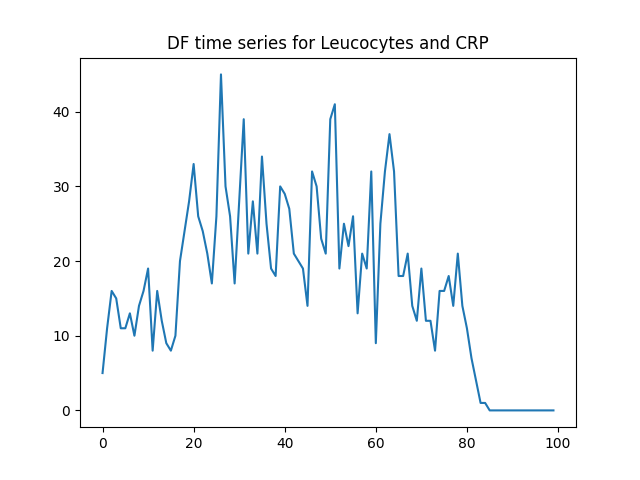
\includegraphics[width=0.49\textwidth]{./img/sepsis_1_t.png}}
	\caption{Sepsis}
	\label{fig:sepsists}
\end{figure}

\begin{figure}[tb]
	\centering
	\subfigure[Most common DF - equisize]{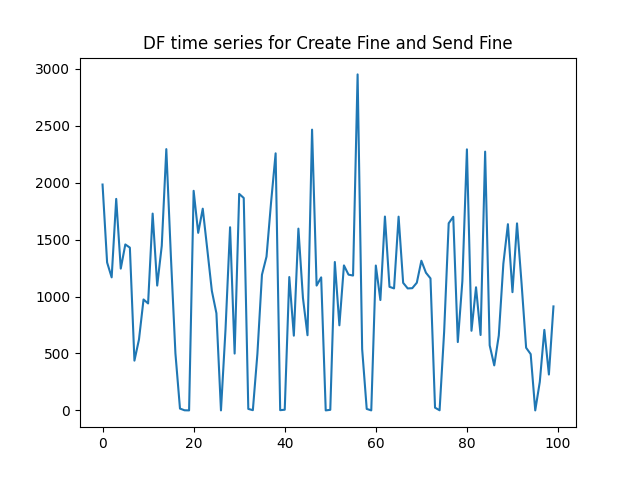
\includegraphics[width=0.49\textwidth]{./img/rtfmp_1.png}}
	\subfigure[Most common DF - equitemp]{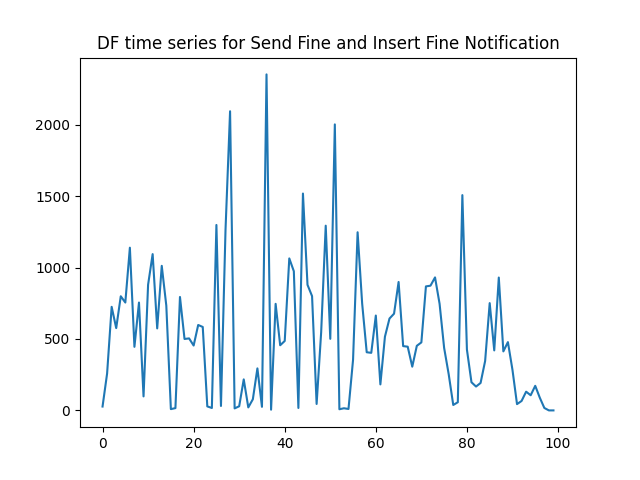
\includegraphics[width=0.49\textwidth]{./img/rtfmp_1_t.png}}
	\caption{RTFMP}
	\label{fig:rtfmpts}
\end{figure}

Resampling is based on a 10-fold cross-validation constructed following a rolling window approach for various horizon values $h\in[1,5]$ where a recursive strategy is used to iteratively obtain $\hat{y}_{t+h|T_{t+h-1}}$ with $(y_1,\dots,y_{T},\dots,\hat{y}_{t+h-1})$ \cite{weigend2018time}.
The 10 training sets exist from $(y_1,\dots,y_{T-h-f})$ and the test sets from\\ $(y_{T-h-f+1},\dots,y_{T-f})$ with $f\in[0,9]$ the fold index \cite{bergmeir2012use}.
While direct strategies with a separate model for every value of $h$ can be used as well and avoid the accumulation of error, they do not take into account statistical dependencies for subsequent predictions.

Given that we want to evaluate the capability of the approach to accurately predict the evolution of the process model, the combination of all DF predictions to obtain a global DFG prediction is considered.
The following two criteria are used:
\begin{itemize}
	\item Cosine distance: measures the distance between two vectors and is often used to compare graph distance. This metric is used to compare the DFG's edge weight matrices between the actual and predicted number of DF relations.
	\item Entropic relevance: a measure for stochastic conformance checking computed as the average number of bits required to compress each of the log’s traces based on the structure and information about relative likelihoods provided by the model \cite{DBLP:conf/icpm/PolyvyanyyMG20}.
\end{itemize}
These criteria balance a predictive and structural evaluation of the algorithms and report on both the numeric performance common in a forecasting setting as well as their appropriateness in terms of reproducing a structurally usable process model which allows for the observed process behavior.

\subsection{Results}
All pre-processing was done in Python with a combination of \emph{pm4py}\footnote{\url{https://pm4py.fit.fraunhofer.de}} and the \emph{statsmodels} package \cite{seabold2010statsmodels}. 
The code is available %TODO here.

The results are displayed in Figures \ref{fig:bpi12_equisize} to \ref{fig:rtfmp_equitemp}.

\begin{figure}
    \centering
    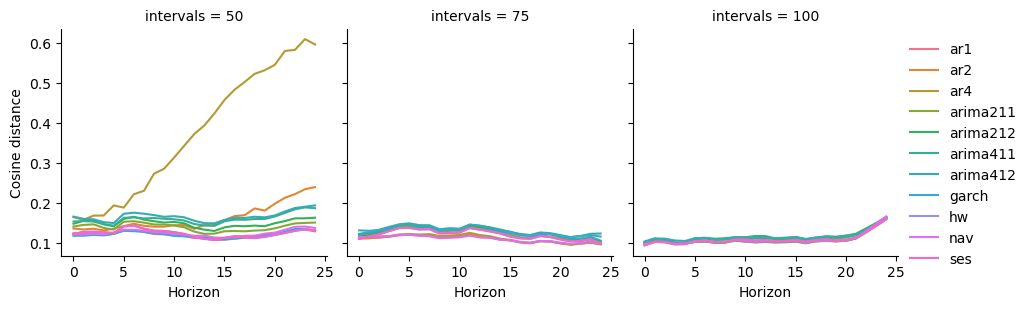
\includegraphics[width=\textwidth]{img/bpi12_cosine_equisize.png}
    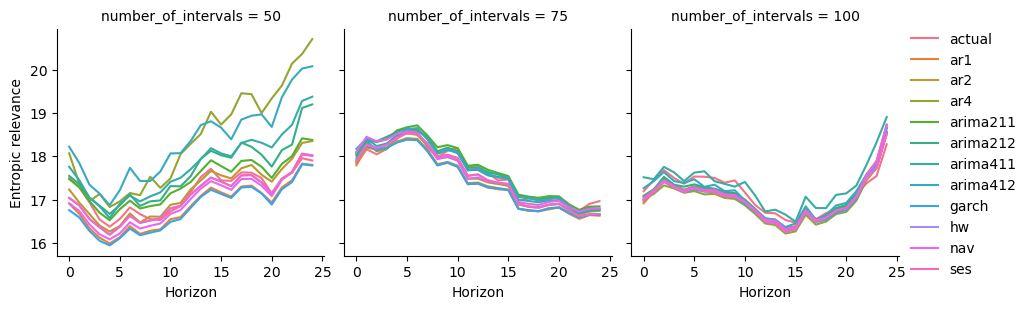
\includegraphics[width=\textwidth]{img/bpi12_entropic_equisize.png}
    \caption{Results for equi-size aggregation for the BPI12 event log.}
    \label{fig:bpi12_equisize}
\end{figure}

\begin{figure}
    \centering
    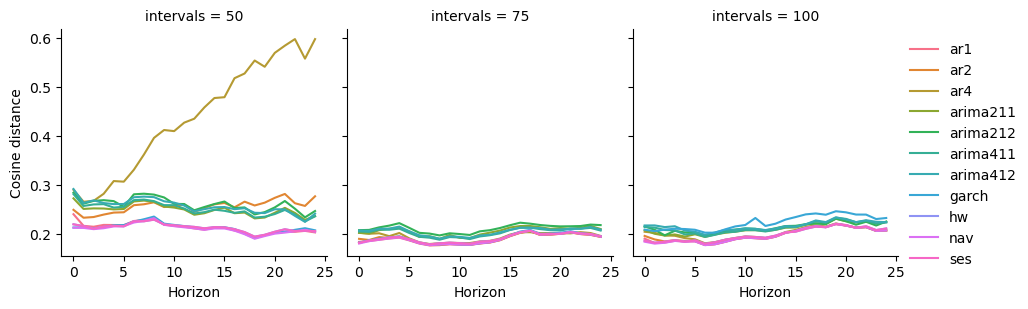
\includegraphics[width=\textwidth]{img/sepsis_cosine_equisize.png}
    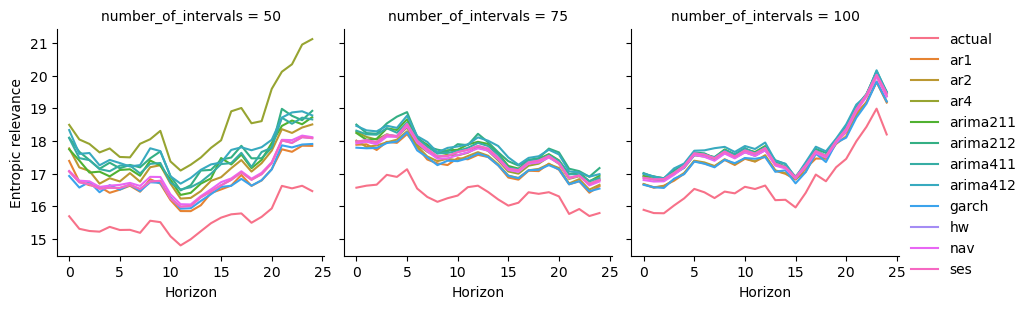
\includegraphics[width=\textwidth]{img/sepsis_entropic_equisize.png}
    \caption{Results for equi-size aggregation for the sepsis event log.}
    \label{fig:sepsis_equisize}
\end{figure}

\begin{figure}
    \centering
    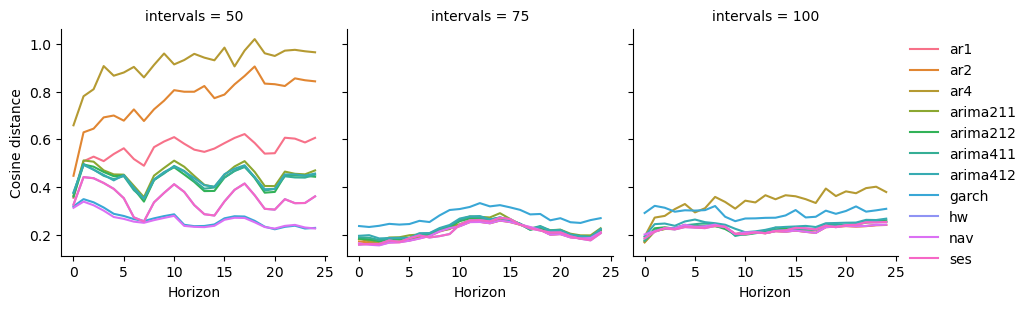
\includegraphics[width=\textwidth]{img/rtfmp_cosine_equisize.png}
    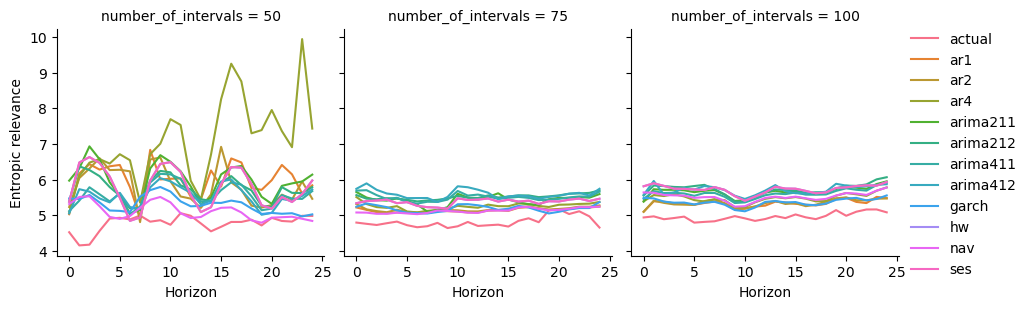
\includegraphics[width=\textwidth]{img/rtfmp_entropic_equisize.png}
    \caption{Results for equi-size aggregation for the RTFMP event log.}
    \label{fig:rtfmp_equisize}
\end{figure}

\begin{figure}
    \centering
    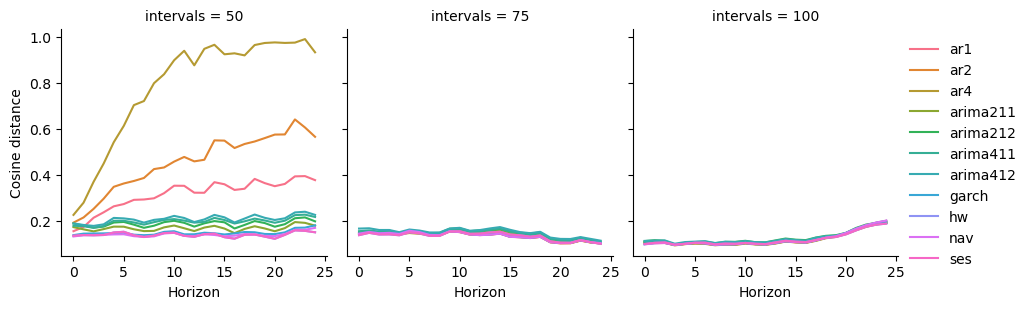
\includegraphics[width=\textwidth]{img/bpi12_cosine_equitemp.png}
    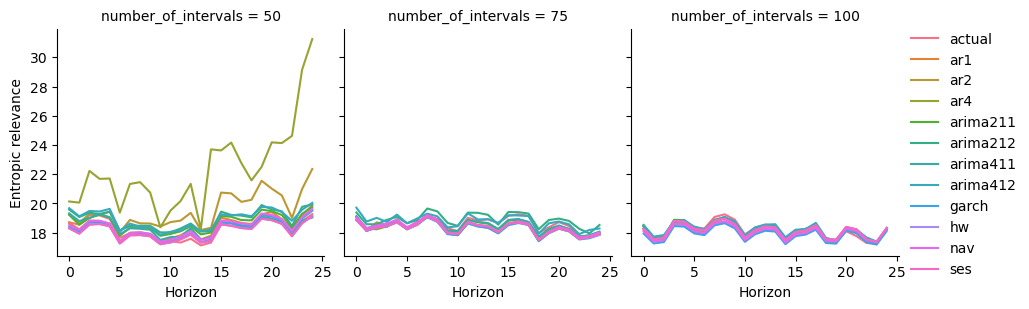
\includegraphics[width=\textwidth]{img/bpi12_entropic_equitemp.png}
    \caption{Results for equi-size aggregation for the BPI12 event log.}
    \label{fig:bpi12_equitemp}
\end{figure}

\begin{figure}
    \centering
    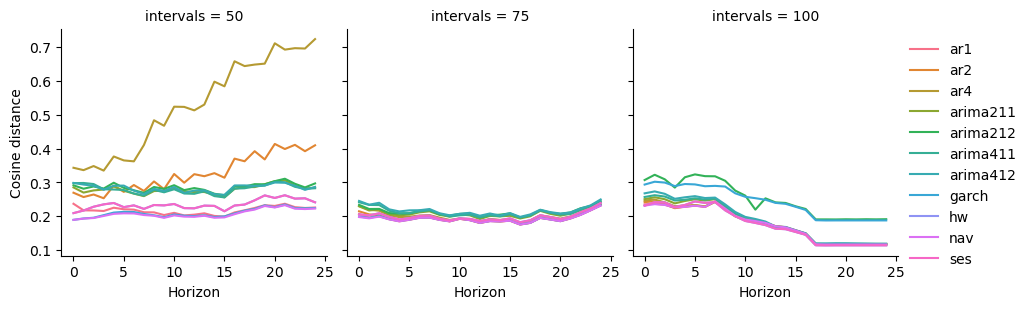
\includegraphics[width=\textwidth]{img/sepsis_cosine_equitemp.png}
    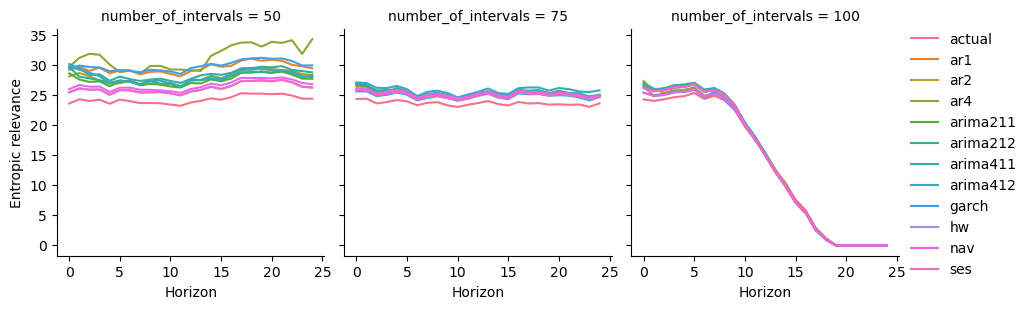
\includegraphics[width=\textwidth]{img/sepsis_entropic_equitemp.png}
    \caption{Results for equi-size aggregation for the sepsis event log.}
    \label{fig:sepsis_equitemp}
\end{figure}

\begin{figure}
    \centering
    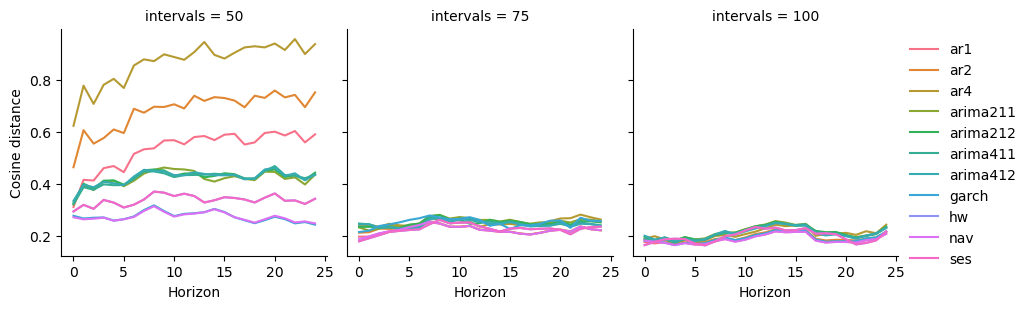
\includegraphics[width=\textwidth]{img/rtfmp_cosine_equitemp.png}
    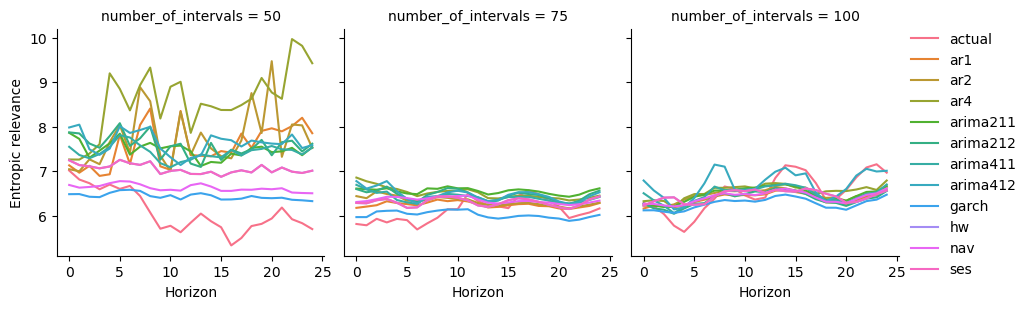
\includegraphics[width=\textwidth]{img/rtfmp_entropic_equitemp.png}
    \caption{Results for equi-size aggregation for the RTFMP event log.}
    \label{fig:rtfmp_equitemp}
\end{figure}


